Sei \(\mathcal{M}^{2k+1}\) eine \(\pi\)-Mannigfaltigkeit, deren Rand entweder leer oder eine Homotopiesph\"are sei. Das Normalenb\"undel einer jeden eingebetteten \(k\)-Sph\"are ist aus Dimensionsgr\"unden \ref{thm:vec_dim_triv} trivial, sodass stets Chirurgie durchgef\"uhrt werden kann. Leider ist \(H_k(\mathcal{M})\) in diesem Fall nicht zwingenderma\ss en frei. Der freie Anteil der Gruppe \(H_k(\mathcal{M})\) ist aufgrund des folgenden Lemmas kein Problem.
\begin{lemma}\label{lem:odd_dim_finite}
    Sei \(\mathcal{M}^{2k+1}\) eine gerahmte Mannigfaltigkeit, sodass \(H^k(\partial\mathcal{M})=0\) ist. Dann kann \(H_k(\mathcal{M})\) durch gerahmte Chirurgie auf ihre Torsionsgruppe reduziert werden.
\end{lemma}
\begin{proof}
    Wenn \(\operatorname{Rang}H_k(\mathcal{M})=0\) gilt, ist die Aussage trivial. Es existiere also ein Generator \(g\) eines direkten \(\mathbb{Z}\)-Summanden von \(H_k(\mathcal{M})\) und ein Homomorphismus \({f\colon H_k(\mathcal{M})\to\mathbb{Z}}\) mit \(f(g)=1\). Aus dem Satz \"uber universelle Koeffizienten folgt, dass \({H^k(\mathcal{M})\to\operatorname{Hom}(H_k(\mathcal{M}),\mathbb{Z})}\) surjektiv ist, sodass ein \(x\in H^k(\mathcal{M})\) mit \(f=\langle x,\mathrel{-}\rangle\) existiert. Aus der Exaktheit der Folge
    \[H^k(\mathcal{M},\partial\mathcal{M})\xrightarrow{q^*}H^k(\mathcal{M})\to H^k(\partial\mathcal{M})=0\]
    folgt, dass auch ein \({h^*\in H^k(\mathcal{M},\partial\mathcal{M})}\) mit \(q^*h^*=x\) existiert. F\"ur das Duale \(h\in H_{k+1}(\mathcal{M})\) folgt
    \[h\cdot g\mathop{=}^{\text{\tiny\eqref{eq:intersect_prop_2}}}\langle q^*h^*,g\rangle=\langle x,g\rangle=f(g)=1\,.\]
    Folglich ist \(g\) primitiv. Da \(g\) von einer eingebetteten Sph\"are mit trivialem Normalenb\"undel repr\"asentiert werden kann, f\"uhrt Chirurgie an \(g\) gem\"a\ss{} Lemma \ref{lem:odd_surg_effect} zu einer Vereinfachung der Homologie. Die Aussage folgt rekursiv.
\end{proof}
Es kann somit angenommen weiter angenommen werden, dass \(H_k(\mathcal{M})\) eine Torsionsgruppe ist. Ob eine Chirurgie die Homologie vereinfacht h\"angt nun von der Parit\"at von \(k\) ab. 

\section{Die Berechnung von \texorpdfstring{\(P^{4m+1}\)}{TEXT}}
    Der am einfachsten zu behandelnde Fall tritt ein, wenn \(k\) gerade ist. Dann ist der Effekt einer Chirurgie an einem Torsionselement, dass dieses durch ein zyklisch unendliches Element ersetzt wird. Somit wird die Gruppe zun\"achst zwar gr\"o\ss er, die Torsionsgruppe wird jedoch definitiv kleiner. Da zyklisch unendliche Elemente mithilfe von Lemma \ref{lem:odd_dim_finite} leicht vernichtet werden k\"onnen, kann auf diese Art und Weise immer eine \(k\)-zusammenh\"angende \(\pi\)-Mannigfaltigkeit erhalten werden. Sei \(\mathbb{K}\) ein K\"orper. Bezeichne
    \[b_i\left(\mathcal{W};\mathbb{K}\right):=\dim_{\mathbb{K}}H_i\left(\mathcal{W};\mathbb{K}\right)\quad\text{und}\quad b_i\left(\mathcal{W},\partial\mathcal{W};\mathbb{K}\right):=\dim_{\mathbb{K}}H_i\left(\mathcal{W},\partial\mathcal{W};\mathbb{K}\right)\,.\]
    F\"ur \(\mathbb{K}=\mathbb{Q}\) ist dies einfach die \(i\)-te Betti-Zahl von \(\mathcal{W}\). Beachte, dass aus der Poincar\'e-Dua\-li\-t\"at bereits \(b_i(\mathcal{W};\mathbb{K})=b_{2\ell-i}(\mathcal{W},\partial\mathcal{W};\mathbb{K})\) folgt. Betrachte zun\"achst folgenden Hilfssatz.
    \begin{lemma}\label{lem:inter_rank_mod}
        Die Schnittpaarung einer Mannigfaltigkeit \(\mathcal{W}^{2\ell}\) mit Werten in einem K\"orper \(\mathbb{K}\) besitzt Rang
        \begin{equation}\label{eq:inter_rank_mod}
            r\equiv\chi(\mathcal{W})+\sum_{i=0}^{\ell-1}b_i\left(\partial\mathcal{W};\mathbb{K}\right)\mod 2\,.
        \end{equation}
    \end{lemma}
    \begin{proof}
        Der Rang der Schnittpaarung ist gerade der Rang der Abbildung
        \[\operatorname{Ad}\colon H_{\ell}(\mathcal{W};\mathbb{K})\to\operatorname{Hom}(H_{\ell}(\mathcal{W};\mathbb{K}),\mathbb{K})\,,\]
        die gem\"a\ss{} Lemma \ref{lem:intersect_factor} gleich der Komposition
        \[H_{\ell}(\mathcal{W};\mathbb{K})\xrightarrow{q_*}H_{\ell}(\mathcal{W},\partial\mathcal{W};\mathbb{K})\xrightarrow{\text{\tiny P.D.}} H^{\ell}(\mathcal{W};\mathbb{K})\xrightarrow{\text{\tiny U.K.}}\operatorname{Hom}(H_{\ell}(\mathcal{W};\mathbb{K}),\mathbb{K})\]
        ist. Da die hinteren beiden Abbildungen Isomorphismen sind, ist der Rang von \(\operatorname{Ad}\) einfach der Rang von \(q_*\). Betrachte die lange exakte Folge
        \[\dots\to H_{\ell}(\mathcal{W};\mathbb{K})\xrightarrow{q_*}H_{\ell}(\mathcal{W},\partial\mathcal{W};\mathbb{K})\xrightarrow{\partial}H_{\ell-1}(\partial\mathcal{W};\mathbb{K})\xrightarrow{\iota_*}H_{\ell-1}(\mathcal{W};\mathbb{K})\to\dots\]
        von \(\mathbb{K}\)-Vektorr\"aumen. Aus dem Rangsatz folgt
        \[\operatorname{Rang}q_*\overeq{Def.}\dim_{\mathbb{K}}\im q_*=\dim_{\mathbb{K}}\ker\partial=\dim_{\mathbb{K}}H_{\ell}(\mathcal{W},\partial\mathcal{W};\mathbb{K})-\operatorname{Rang}\partial\,,\]
        sodass sich induktiv ergibt, dass \(\operatorname{Rang}q_*\) die alternierende Summe der Dimensionen aller Vektorr\"aume rechts von \(H_{\ell}(\mathcal{W},\partial\mathcal{W};\mathbb{K})\) ist. Modulo zwei ist also
        \[\operatorname{Rang}q_*\equiv\sum_{i=0}^{\ell-1}b_i\left(\mathcal{W};\mathbb{K}\right)+\sum_{i=0}^{\ell-1}b_i\left(\partial\mathcal{W};\mathbb{K}\right)+\sum_{i=0}^{\ell}b_i(\mathcal{W},\partial\mathcal{W};\mathbb{K})\mod2\,.\]
        Wegen \(b_i(\mathcal{W},\partial\mathcal{W};\mathbb{K})=b_{2\ell-i}\left(\mathcal{W};\mathbb{K}\right)\) folgt weiter
        \[\operatorname{Rang}q_*\equiv\sum_{i=0}^{2\ell}b_i\left(\mathcal{W};\mathbb{K}\right)+\sum_{i=0}^{\ell-1}b_i\left(\partial\mathcal{W};\mathbb{K}\right)\equiv\chi(\mathcal{W})+\sum_{i=0}^{\ell-1}b_i\left(\partial\mathcal{W};\mathbb{K}\right)\mod2\,.\]
    \end{proof}
    \begin{lemma}\label{lem:srg_chg_field_betti}
        Sei \(\mathbb{K}\) ein K\"orper, \(\mathcal{M}^{2k+1}\) eine \((k-1)\)-zusammenh\"angende, geschlossene Mannigfaltigkeit und \({\mathcal{W}^{2k+2}:=\mathcal{M}\times\mathbb{I}\multimap\mathbb{D}^{k+1}}\), sodass die Schnittform von \(\mathcal{W}\) geraden Rang besitzt. Dann gilt \(b_k(\mathcal{M};\mathbb{K})\not=b_k(\mathcal{M}\multimap\mathbb{S}^k;\mathbb{K})\).
    \end{lemma}
    \begin{proof}
        Setze \(\mathcal{M}^{\prime}:=\mathcal{M}\multimap\mathbb{S}^k\). Die Euler-Cha\-rak\-te\-ris\-tik einer kompakten Mannigfaltigkeit ungerade Dimension (mit oder ohne Rand) ist gleich null. Da \(\mathcal{W}\) homotopie\"aquivalent zu \(\mathcal{M}\) mit einer \((k+1)\)-Zelle ist, gilt also
        \begin{equation}\label{eq:w_euler}
            \chi(\mathcal{W})=\chi(\mathcal{M})+(-1)^{k+1}=(-1)^{k+1}\,.
        \end{equation}
        Da die Schnittpaarung auf \(\mathcal{W}\) geraden Rang besitzt, folgt
        \begin{equation}\label{eq:betti_cong}
            \begin{array}{rll}
                0\hspace{-2pt}&\displaystyle\hspace{-4pt}\mathop{\equiv}^{\text{\tiny\eqref{eq:inter_rank_mod}}}\chi(\mathcal{W})+\sum_{i=0}^k\big(b_i\left(\mathcal{M};\mathbb{K}\right)+b_i\left(\mathcal{M}^{\prime};\mathbb{K}\right)\big)&\mod2\\
                &\displaystyle\hspace{-4pt}\mathop{\equiv}^{\text{\tiny\eqref{eq:w_euler}}}1+\sum_{i=0}^kb_i\left(\mathcal{M};\mathbb{K}\right)+\sum_{i=0}^kb_i\left(\mathcal{M}^{\prime};\mathbb{K}\right)&\mod2\,.
            \end{array}
        \end{equation}
        Da \(\mathcal{M}\) und \(\mathcal{M}^{\prime}\) jeweils \((k-1)\)-zusammenh\"angend sind, zeigt dies
        \[b_k\left(\mathcal{M};\mathbb{K}\right)=\sum_{i=1}^kb_i\left(\mathcal{M};\mathbb{K}\right)\mathop{\neq}^{\text{\tiny\eqref{eq:betti_cong}}}\sum_{i=1}^kb_i\left(\mathcal{M}^{\prime};\mathbb{K}\right)=b_k\left(\mathcal{M}^{\prime};\mathbb{K}\right)\,.\]
    \end{proof}
    \begin{corollary}\label{cor:srg_chg_betti}
        Ist \(k\) gerade und \(\mathcal{M}^{2k+1}\) eine Mannigfaltigkeit, deren Rand leer oder eine Homotopiesph\"are ist, ver\"andert eine \(k\)-Chirurgie die \(k\)-te Betti-Zahl.
    \end{corollary}
    \begin{proof}
        Ist \(\mathcal{M}\) geschlossen, folgt dies aus Lemma \ref{lem:srg_chg_field_betti}, da die Schnittform auf \(\mathcal{M}\times\mathbb{I}\multimap\mathbb{D}^{k+1}\) schiefsymmetrisch ist, und deshalb geraden Rang besitzt. Sei nun \(\partial\mathcal{M}\) eine Homotopiesph\"are. Betrachte die geschlossene Mannigfaltigkeit
        \[\mathcal{N}:=\mathcal{M}\mathop{+}^{\partial\mathcal{M}}\mathcal{M}\,.\]
        Dann gelten
        \[H_k(\mathcal{N})\cong H_k(\mathcal{M})\oplus H_k(\mathcal{M})\quad\text{und}\quad H_k(\mathcal{N}\multimap\mathbb{S}^k)\cong H_k(\mathcal{M})\oplus H_k(\mathcal{M}\multimap\mathbb{S}^k)\,.\]
        Also \(b_k(\mathcal{N})=2b_k(\mathcal{M})\) und \(b_k(\mathcal{N}\multimap\mathbb{S}^k)=b_k(\mathcal{M})+b_k(\mathcal{M}^{\prime})\). Da der Satz f\"ur geschlossene Mannigfaltigkeiten bereits gezeigt wurde, folgt
        \[2b_k(\mathcal{M})\not=b_k(\mathcal{M})+b_k(\mathcal{M}^{\prime})\quad\text{also}\quad b_k(\mathcal{M})\not=b_k(\mathcal{M}^{\prime})\,.\]
    \end{proof}
    Damit sind bereits alle notwendigen Werkzeuge gegeben um \(P^{4m+1}\) zu berechnen.
    \begin{theorem}\label{thm:4m+1}
        Eine gerahmte Mannigfaltigkeit \(\mathcal{M}^{4m+1}\), deren Rand leer oder eine Homotopiesph\"are ist, ist zu einer \(k\)-zusammenh\"angenden gerahmten Mannigfaltigkeit \(\chi\)-\"aquivalent.
    \end{theorem}
    \begin{proof}
        Aus Lemma \ref{lem:odd_dim_finite} folgt, dass \(\mathcal{M}^{2k}\) als \((k-1)\)-zu\-sam\-men\-h\"ang\-end und \(H_k(\mathcal{M})\) als endlich angenommen werden kann, also Betti-Zahl null besitzt. Ist \(H_k(\mathcal{M})=0\) ist die Aussage trivial. Es existiere also ein nicht-triviales Element in \(H_k(\mathcal{M})\), welches durch eine eingebettete Sph\"are \(\mathcal{S}\) repr\"asentiert wird, die gem\"a\ss{} Satz \ref{thm:vec_dim_triv} ein triviales Normalenb\"undel besitzt. Eine Chirurgie an \(\mathcal{S}\) ergibt gem\"a\ss{} Korollar \ref{cor:srg_chg_betti} eine Mannigfaltigkeit \(\mathcal{M}^{\prime}\) mit Betti-Zahl ungleich null. Da 
        \[H_k(\mathcal{M})/\langle\eqcl{e\mathrel{|}\mathcal{M}}\rangle\cong H_k(\mathcal{M}^{\prime})/\langle\eqcl{m\mathrel{|}\mathcal{M}^{\prime}}\rangle\]
        gilt, die linke Gruppe endlich ist und \(H_k(\mathcal{M}^{\prime})\) mindestens einen direkten \(\mathbb{Z}\)-Sum\-man\-den besitzt, muss \(\langle\eqcl{m\mathrel{|}\mathcal{M}^{\prime}}\rangle\cong\mathbb{Z}\) sein. Dies zeigt, dass die Torsionsuntergruppe von \(H_k(\mathcal{M}^{\prime})\) zu einer Untergruppe von \(H_k(\mathcal{M})/\langle\eqcl{e\mathrel{|}\mathcal{M}}\rangle\) isomorph ist. Da \(\mathcal{M}^{\prime}\) erneut durch Chirurgie in eine Mannigfaltigkeit \"uberf\"uhrt werden kann, deren \(k\)-te Homologiegruppe die Torsionsuntergruppe von \(H_k(\mathcal{M}^{\prime})\) ist, kann \(H_k(\mathcal{M})\) durch zwei Chirurgien durch eine definitiv kleinere endliche Gruppe ersetzt werden. Die Aussage folgt rekursiv.
    \end{proof}

    \begin{corollary}\label{cor:double_odd_zero}
        Es gilt \(P^{4m+1}\cong0\).
    \end{corollary}

\section{Die Berechnung von \texorpdfstring{\(P^{4m+3}\)}{TEXT}}
    Sei \(k\) nun ungerade und \(\mathcal{M}^{2k}\) eine \((k-1)\)-zusammenh\"angende \(\pi\)-Man\-nig\-fal\-tig\-keit, sodass \(H_k(\mathcal{M})\) endlich ist. Sei \(x\in H_k(\mathcal{M})\) und \(\mathcal{S}\) eine repr\"asentierende Sph\"are. Aus Dimensionsgr\"unden \ref{thm:vec_dim_triv} ist das Normalenb\"undel von \(\mathcal{S}\subseteq\mathring{\mathcal{M}}\) trivial, sodass eine gerahmte Chirurgie an \(\mathcal{S}\) durchgef\"uhrt werden kann. Das Problem in dieser Dimension besteht darin, dass eine derartige Chirurgie die Homologie nicht zwingenderma\ss en vereinfacht. Um dem beizukommen ist eine weitere sorgsame Reparametrisierung vonn\"oten. 
    \subsubsection{Effekt einer Reparametrisierung auf \(H_k(\mathcal{M}_0)\)}
        Sei \({\Phi\colon\underline{\mathbb{D}}^{k+1}\hookrightarrow\mathring{\mathcal{M}}}\) eine Anklebeeinbettung, \({\mathcal{D}:=\im\Phi}\) und \({\mathcal{M}_0:=\mathcal{M}\setminus\mathring{\mathcal{D}}}\). Sei \(\mathcal{M}^{\prime}\) die Chirurgie und \(\mathcal{M}_{\gamma}^{\prime}\) die mit einem \(\gamma\colon\mathbb{S}^k\to\operatorname{SO}(k+1)\) reparametrisierte Chirurgie. Beachte, dass \({\partial\mathcal{D}\cong\mathbb{S}^k\times\mathbb{S}^k}\) gilt. Seien \(e,m\in H_k(\mathbb{S}^k\times\mathbb{S}^k)\) die Fundamentalklassen eines \"Aquators \({\mathbb{S}^k\times y}\) und eines Meridians \({x\times\mathbb{S}^k}\). Sei
        \[\overline{\Gamma}\colon\mathbb{S}^k\times\mathbb{S}^k\to\mathbb{S}^k\times\mathbb{S}^k,\,(x,y)\mapsto(x,\gamma(x)\cdot y)\]
        die zugeh\"orige Reparametrisierungsabbildung. Dann folgt \"uber den Satz von Hurewicz, dass in \(H_k(\mathbb{S}^k\times\mathbb{S}^k)\) die Gleichungen
        \begin{equation}\label{eq:torus_reparam}
            e^{\gamma}:=\overline{\Gamma}_*e=e+\psi_*(\eqcl{\gamma})\,m\quad\text{und}\quad\overline{\Gamma}_*m=m\,.
        \end{equation}
        gelten. Es folgt, dass dies auch f\"ur die Inkludierten \(e_0\), \(e_0^{\gamma}\) und \(m_0\) in \(H_k(\mathcal{M}_0)\) gilt. Wie zuvor kann stets eine Reparametrisierung mit einem Element des Kernes der iterierten Einh\"angung \(S_*^{k+1}\) vorgenommen werden. Aus Stabilisierungsgr\"unden ist dies gerade die rechte Abbildung in dem Diagramm
        \begin{center}
            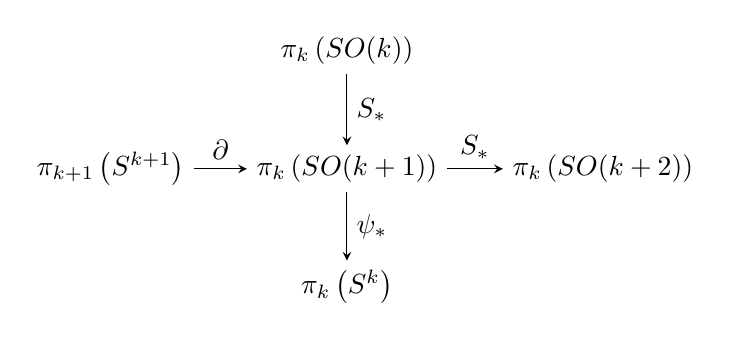
\begin{tikzpicture}
                \draw
                    (-3, 0) node (A) {\(\pi_{k+1}\left(\mathbb{S}^{k+1}\right)\)}
                    (0, 0) node (B) {\(\pi_k\left(\operatorname{SO}(k+1)\right)\)}
                    (3.25, 0) node (C) {\(\pi_k\left(\operatorname{SO}(k+2)\right)\)}
                    (0, 1.5) node (D) {\(\pi_k\left(\operatorname{SO}(k)\right)\)}
                    (0, -1.5) node (E) {\(\pi_k\left(\mathbb{S}^k\right)\)}
                    
                    (A) edge [-stealth] node [above] {\(\partial\)} (B)
                    (B) edge [-stealth] node [above] {\(S_*\)} (C)
                    
                    (D) edge [-stealth] node [right] {\(S_*\)} (B)
                    (B) edge [-stealth] node [right] {\(\psi_*\)} (E)
                    ;
            \end{tikzpicture}
        \end{center}
        Erneut wird \(\ker S_*\) wird von dem Tangentialb\"undel der Sph\"are erzeugt, und ist f\"ur gerade \(k\) zyklisch unendlich. Diese wird unter \(\psi_*\) auf das Doppelte eines Erzeugers abgebildet. Somit kann \(\psi_*\eqcl{\gamma}\) als jedes beliebige Vielfache von \(2\) gew\"ahlt werden.

    \subsubsection{Effekt einer Reparametrisierung auf den Rang von \(H_k(\mathcal{M}^{\prime})\)}
        Seien \(e^{\prime}\in H_k(\mathcal{M})\), \(m^{\prime}\in H_k(\mathcal{M}^{\prime})\) und \(m_{\gamma}^{\prime}\in H_k(\mathcal{M}_{\gamma}^{\prime})\). Sei \(\ell\) der Rang von \(e^{\prime}\). Dann folgt aus der exakten Folge
        \[0\to\mathbb{Z}\xrightarrow{\lambda}H_k(\mathcal{M}_0)\to H_k(\mathcal{M})\to0\,,\]
        dass \(\ell e_0\in\im\lambda\) liegt. Dieses Bild besteht gerade aus den Vielfachen von \(m_0\), also existiert eine Abh\"angigkeit
        \[\ell e_0+\ell^{\prime}m_0=0\,.\]
        Hierbei ist \(\ell^{\prime}\) der Rang von \(m^{\prime}\). Wegen \(e_0^{\gamma}=e_0+\psi_*(\eqcl{\gamma})m_0\) folgt
        \[0=\ell e_0+\ell^{\prime}m_0=\ell\left(e_0^{\gamma}-\psi_*(\eqcl{\gamma})m_0\right)+\ell^{\prime}m_0=\ell e_0^{\gamma}+\left(\ell^{\prime}-\ell\psi_*(\eqcl{\gamma})\right)m_0\,.\]
        Folglich besitzt \(m_{\gamma}^{\prime}\) den Rang \(\abs{\ell^{\prime}-\ell\psi_*(\eqcl{\gamma})}\). Da weiterhin
        \[H_k(\mathcal{M}_{\gamma}^{\prime})/\langle m_{\gamma}^{\prime}\rangle\cong H_k\left(\mathcal{M}\right)/\langle e^{\prime}\rangle\]
        gilt, ist \(H_k(\mathcal{M}_{\gamma}^{\prime})\) kleiner als \(H_k\left(\mathcal{M}\right)\), wenn \(0\leq\operatorname{Rang}m_{\gamma}^{\prime}<\operatorname{Rang}e^{\prime}\) also
        \[0\leq\abs{\ell^{\prime}-\ell\psi_*(\eqcl{\gamma})}<\ell\]
        ist. Da \(\eqcl{\gamma}\in\ker S_*\) so gew\"ahlt werden kann, dass \(\psi_*(\eqcl{\gamma})\) eine beliebige gerade Zahl ist, kann dies, insofern \(\ell^{\prime}\) nicht von \(\ell\) geteilt wird, stets m\"oglich. Um das Teilungsverhalten von \(\ell^{\prime}\) und \(\ell\) zu untersuchen wird die Verschlingungszahl ben\"otigt.

    \subsubsection{Die Verschlingungszahl}
        Sei \(\mathcal{M}^n\) eine orientierte Mannigfaltigkeit und \(n=i+j+1\). Die kurze exakte Folge von Kettenkomplexen
        \[0\to C_*\left(\mathcal{M};\mathbb{Z}\right)\mathop{\rightarrowtail}^pC_*\left(\mathcal{M};\mathbb{Q}\right)\twoheadrightarrow C_*\left(\mathcal{M};\mathbb{Q}/\mathbb{Z}\right)\to0\]
        induziert eine lange exakte Folge
        \[H_{i+1}\left(\mathcal{M};\mathbb{Q}/\mathbb{Z}\right)\xrightarrow{\partial}H_i\left(\mathcal{M};\mathbb{Z}\right)\xrightarrow{p_*}H_i\left(\mathcal{M};\mathbb{Q}\right)\to H_i\left(\mathcal{M};\mathbb{Q}/\mathbb{Z}\right)\]
        Seien \(x\in H_i(\mathcal{M})\) und \(y\in H_j(\mathcal{M})\) endlichen Ranges. Dann gilt \(p_*x=0\), sodass \(x\) zu einem \(\mu\in H_{i+1}(\mathcal{M};\mathbb{Q}/\mathbb{Z})\) mit \(\partial\mu=x\) zur\"uckgezogen werden kann. Definiere die \textbf{Verschlingungszahl} (Linking number) von \(x\) und \(y\) als Schnittzahl repr\"a\-sen\-tie\-ren\-der Ketten von \(x\) mit \(\mu\). Die derart erhaltene Bilinearform ist nicht entartet, und es gilt
        \[L(x,y)+(-1)^{ij}L(y,x)\,.\]
        \begin{lemma}
            Sei \(k>1\) ungerade und \(\mathcal{M}^{2k+1}\) eine Mannigfaltigkeit, sodass \(H_k(\mathcal{M})\) endlich ist. Wird \(x\in H_k(\mathcal{M})\) vom Rang \(\ell\) durch Chirurgie an \(x\) durch ein Element vom Rang \(\ell^{\prime}\) ersetzt, gilt \(\ell^{\prime}/\ell=\pm L(x,x)\in\mathbb{Q}/\mathbb{Z}\).
        \end{lemma}
        \begin{proof}
            Sei \(z_1,z_2\in C_k(\mathcal{M}_0)\) Zyklen, die \(e_0\) und \(m_0\) repr\"asentieren. Wegen \(0=\ell e_0+\ell^{\prime}m_0\), existiert eine Kette \(c\in C_{k+1}(\mathcal{M}_0)\) mit
            \[\partial c=\ell z_1+\ell^{\prime}z_2\,.\]
            Sei \(c_1\in C_{k+1}(\mathcal{M})\) der durch \(\Phi(x\times\mathbb{D}^{k+1})\) definierte Zyklus mit \(\partial c_1=z_2\). Ist \(c_2\) jene durch \(\Phi(\mathbb{S}^k\times0)\) definierte Kette, die \(e\) repr\"asentiert, so gilt
            \[\partial(c-\ell^{\prime}c_1)/\ell=z_1\quad\text{und somit}\quad L(e,e)=(c-\ell^{\prime}c_1)/\ell\cdot c_2\,,\]
            Da \(c_2\) und \(c\) disjunkt sind gilt \(c\cdot c_2=0\), und da \(c_1\) und \(c_2\) genau einen Schnittpunkt in \((x,0)\) besitzen gilt \(c_1\cdot c_2=\mp1\). Es folgt \(L(e,e)=\mp\ell^{\prime}/\ell\).
        \end{proof}
        \begin{corollary}\label{cor:link_nzero_small}
            Sei \(k>1\) ungerade und \(\mathcal{M}^{2k+1}\) eine gerahmte Mannigfaltigkeit, sodass \(H_k(\mathcal{M})\) endlich ist. Existiert ein \(x\in H_k(\mathcal{M})\) mit \(L(x,x)\not=0\), kann \(H_k(\mathcal{M})\) durch eine gerahmte Chirurgie verkleinert werden. 
        \end{corollary}
        Auf diese Art und Weise kann \(H_k(\mathcal{M})\) so lange weiter verkleinert werden, bis keine \(x\) mit \(L(x,x)\not=0\) mehr existieren. Dann besitzt die Gruppe wegen folgendem Lemma jedoch eine besonders einfache Struktur.
        \newpage
        \begin{lemma}\label{lem:link_z2}
            Sei \(k>1\) ungerade und \(\mathcal{M}^{2k+1}\) eine Mannigfaltigkeit, sodass \(H_k(\mathcal{M})\) endlich ist. Gilt \(L(x,x)=0\) f\"ur alle \(x\in H_k(\mathcal{M})\), ist \(H_k(\mathcal{M})\cong\mathbb{Z}_2^{\oplus s}\).
        \end{lemma}
        \begin{proof}
            Aus \({L(\epsilon,\delta)+(-1)^kL(\delta,\epsilon)=0}\) folgt, dass die Verschlingungspaarung f\"ur \({i=j}\) symmetrisch ist. Da \(L(x,x)=0\) f\"ur alle \(x\in H_k(\mathcal{M})\) gilt, ergibt sich
            \[0=L(\epsilon+\delta,\epsilon+\delta)=L(\epsilon,\epsilon)+2L(\epsilon,\delta)+L(\delta,\delta)=2L(\epsilon,\delta)\,.\]
            Da die Verschlingungspaarung nicht entartet ist, folgt aus \(L(2\epsilon,\delta)=0\) f\"ur alle \(\delta\) bereits \(2\epsilon=0\).
        \end{proof}
        \begin{lemma}\label{lem:rep_group}
            Sei \(k>1\) ungerade. Ist \(\mathcal{M}^{2k+1}\) eine geschlossene \((k-1)\)-zu\-sam\-men\-h\"an\-gen\-de gerahmte Mannig\-faltig\-keit mit \(H_k(\mathcal{M})\cong\mathbb{Z}_2^{\oplus s}\), kann eine gerahmte Chirurgie an \(\mathcal{M}\) durchgef\"uhrt werden, sodass 
            \begin{equation}\label{eq:surg_poss}
                H_k(\mathcal{M}^{\prime})\cong\mathbb{Z}\oplus\mathbb{Z}_2^{\oplus(s-2)}\quad\text{oder}\quad H_k(\mathcal{M}^{\prime})\cong\mathbb{Z}_4\oplus\mathbb{Z}_2^{\oplus(s-2)}
            \end{equation}
            ist.
        \end{lemma}
        \begin{proof}
            Sei \(x\in H_k(\mathcal{M})\). Setze \({\mathcal{W}:=\mathcal{M}\times\mathbb{I}\multimap\mathbb{D}^{k+1}}\) und \({\mathcal{M}^{\prime}:=\mathcal{M}\multimap\mathbb{S}^k}\) sodass die Anklebesph\"are \(x\) repr\"asentiere. F\"ur das \(k\)-te Steenrod-Quadrat gilt
            \[\operatorname{Sq}^k\colon H^{k+1}(\mathcal{W},\partial\mathcal{W};\mathbb{F}_2)\to H^{2k+1}(\mathcal{W},\partial\mathcal{W};\mathbb{F}_2)\cong H_1(\mathcal{W};\mathbb{F}_2)=0\]
            sodass aus der Adem-Beziehung \({\operatorname{Sq}^{k+1}=\operatorname{Sq}^1\smile\operatorname{Sq}^k}\) bereits \(\operatorname{Sq}^{k+1}=0\) folgt. Dies zeigt f\"ur alle \(x\in H_{k+1}(\mathcal{W};\mathbb{F}_2)\) die Gleichung
            \[x\cdot x=\left\langle x^*\smile x^*,\eqcl{\mathcal{W}}\right\rangle=\big\langle\operatorname{Sq}^{k+1}(x^*),\eqcl{\mathcal{W}}\big\rangle=0\,,\]
            sodass die Schnittform auf \(H_{k+1}(\mathcal{W};\mathbb{F}_2)\) geraden Rang besitzt. Gem\"a\ss{} Lemma \ref{lem:srg_chg_field_betti} folgt, dass \(\dim_{\mathbb{F}_2}H_k(\mathcal{M}^{\prime};\mathbb{F}_2)\not=\dim_{\mathbb{F}_2}H_k(\mathcal{M};\mathbb{F}_2)\) gilt. Eine Chirurgie kann wie zuvor so reparametrisiert werden, dass \(x\) durch ein Element \(x^{\prime}\in H_k(\mathcal{M}^{\prime})\) geraden Ranges \(\ell^{\prime}\) mit \(0\leq\ell^{\prime}\leq2\) ersetzt wird. Somit ist \(\ell^{\prime}\) entweder null oder zwei. Aus
            \[H_k(\mathcal{M}^{\prime})/\langle x^{\prime}\rangle\cong H_k(\mathcal{M})/\langle x\rangle\cong\mathbb{Z}_2^{\oplus(s-1)}\]
            folgt die Existenz einer kurzen exakten Folge
            \[0\to\mathbb{Z}_{\ell^{\prime}}\rightarrowtail H_k(\mathcal{M}^{\prime})\twoheadrightarrow\mathbb{Z}_2^{\oplus(s-1)}\to0\,.\]
            Beachte \({\mathbb{Z}_0\cong\mathbb{Z}}\). W\"urde diese spalten, g\"olte \({H_k(\mathcal{M}^{\prime};\mathbb{F}_2)\cong\mathbb{Z}_2\oplus\mathbb{Z}_2^{\oplus(s-1)}}\), was ein Widerspruch gegen den Fakt w\"are, dass die Chirurgie die \(\mathbb{F}_2\)-Dimension ver\"andert. Folglich bleiben lediglich die M\"og\-lich\-kei\-ten aus Gleichung \ref{eq:surg_poss}.
        \end{proof}
        \newpage
        \begin{lemma}\label{lem:link_zero_small}
            Sei \(k>1\) ungerade und \(\mathcal{M}^{2k+1}\) eine \((k-1)\)-zu\-sam\-men\-h\"an\-gen\-de gerahmte Man\-nig\-fal\-tig\-keit, deren Rand leer oder eine Homotopiesph\"are ist sodass \(H_k(\mathcal{M})\) endlich ist. Existiert \textbf{kein} \(x\in H_k(\mathcal{M})\) mit \(L(x,x)\not=0\), kann \(H_k(\mathcal{M})\) trotzdem durch eine gerahmte Chirurgie verkleinert werden.
        \end{lemma}
        \begin{proof}
            Da \(L(x,x)=0\) f\"ur alle \(x\in H_k(\mathcal{M})\) gilt, folgt aus Lemma \ref{lem:link_z2} \(H_k(\mathcal{M})\cong\mathbb{Z}_2^{\oplus s}\). Dann ist 
            \[\mathcal{N}:=\mathcal{M}\mathop{+}^{\partial\mathcal{M}}\mathcal{M}\quad\text{mit}\quad{H_k(\mathcal{N})}\cong H_k(\mathcal{M})\oplus H_k(\mathcal{M})\cong\mathbb{Z}_2^{\oplus2s}\]
            eine geschlossene Mannigfaltigkeit. Gem\"a\ss{} Lemma \ref{lem:rep_group} kann an \(\mathcal{N}\) eine Chirurgie durchgef\"uhrt werden, sodass 
            \[\mathbb{Z}_2^{\oplus s}\oplus H_k(\mathcal{M}\multimap\mathbb{S}^k)\cong H_k(\mathcal{N}\multimap\mathbb{S}^k)\cong\mathbb{Z}_2^{\oplus s}\oplus\begin{cases}
                \mathbb{Z}\oplus\mathbb{Z}_2^{\oplus(s-2)}\\
                \mathbb{Z}_4\oplus\mathbb{Z}_2^{\oplus(s-2)}
            \end{cases}\]
            gilt. Da \(\mathbb{Z}_2^{\oplus s}\) gek\"urzt werden kann, ist \(H_k(\mathcal{M}\multimap\mathbb{S}^k)\) entweder zu \(\mathbb{Z}_4\oplus\mathbb{Z}_2^{\oplus(s-2)}\) oder zu \(\mathbb{Z}\oplus\mathbb{Z}_2^{\oplus(s-2)}\) isomorph. Im ersten Fall ergibt dies direkt eine kleinere Gruppe als \(H_k(\mathcal{M})\), im zweiten Fall muss vorher der direkte \(\mathbb{Z}\)-Summand mithilfe von Lemma \ref{lem:odd_dim_finite} eliminiert werden. 
        \end{proof}
        Aus Korollar \ref{cor:link_nzero_small} und Lemma \ref{lem:link_zero_small} folgt zusammen:
        \begin{corollary}\label{cor:single_odd_zero}
            Es gilt \(P^{4m+3}=0\).
        \end{corollary}